%***************************************PREAMBLE***************************************
\documentclass[a4paper,12pt]{article}

\usepackage[utf8]{inputenc}
\usepackage[margin=0.7in]{geometry}
\usepackage[T1]{fontenc}
\usepackage{graphicx}
\usepackage{float}
\usepackage{setspace}
\usepackage{appendix}
\usepackage{amsmath}
\usepackage{amssymb}
\usepackage{cite}
\usepackage{caption}
\usepackage{subcaption}


%***************************************DOCUMENT***************************************

\DeclareMathOperator*{\argmin}{\arg\!\min}
\DeclareMathOperator*{\argmax}{\arg\!\max}

\graphicspath{ {./images/} }
\setlength{\parindent}{0pt}

\begin{document}
	\fontfamily{ptm}\selectfont
	%%%%%%%%%%%%%%%%%%%%%%%%%%%%%%%%%%%%%%%COVERSHEET%%%%%%%%%%%%%%%%%%%%%%%%%%%%%%%%%%%%%%%
	\begin{titlepage}
		\setlength{\voffset}{-0.8in}
		\noindent \makebox[\textwidth]{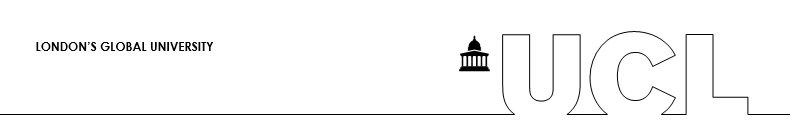
\includegraphics[width=1.2\textwidth]{Coversheet_Header.png}}
	
			\vspace{15mm}
			
			\begin{center}
				{\Huge \textbf{COMP0037 \\ \vspace{10mm} Report}}
			
				\vspace{8mm}
			
				\begin{spacing}{1.8}
					{\huge Planning in Uncertain Worlds}
				\end{spacing}
		
			
				\vspace{12mm}
			
				{\LARGE \textbf{Group AS}}
				
				\vspace{10mm}
				
				\begin{tabular}{ll}
					\underline{\textbf{Student Name}}  & \hspace{4mm} \underline{\textbf{Student number}} \vspace{2mm} \\
					Arundathi Shaji Shanthini & \hspace{4mm} 16018351 \\ 
					Dmitry Leyko & \hspace{4mm}  16021440\\ 
					Tharmetharan Balendran & \hspace{4mm} 17011729\\ 
				\end{tabular}
				
				\vspace{13mm}
				
				\begin{tabular}{ll}
					\textbf{Department:} &  Department of Electronic and Electrical Engineering\\ \vspace{3mm}
					\textbf{Submission Date:} &  28\textsuperscript{th} of April 2020
				\end{tabular}
			\end{center}
	\end{titlepage}
	%%%%%%%%%%%%%%%%%%%%%%%%%%%%%%%%%%%%%%
	
	\pagebreak
	
	\tableofcontents
	
	\pagebreak
	
	%%%%%%%%%%% PART 1 %%%%%%%%%%%%%%%%%
	\section{Decision Re-Plan Policy}
	\label{sec:decisionReplanPolicy}

		\subsection{Policy Selection when Obstacle is Observed}
		\label{sec:policySelectionWhenObstacleIsObserved}
		
			\begin{figure}[H]
				\centering
				\begin{subfigure}{.4\textwidth}
					\centering
					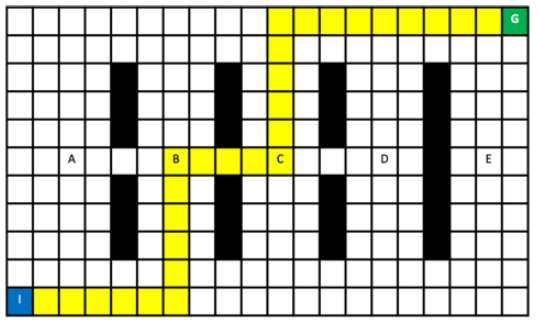
\includegraphics[width=\linewidth]{originalPlannedPath.png}
					\caption{The original planned path form I to G going through Aisle B and C.}
					\label{fig:originalPlannedPath}
				\end{subfigure}
				\begin{subfigure}{.4\textwidth}
					\centering
					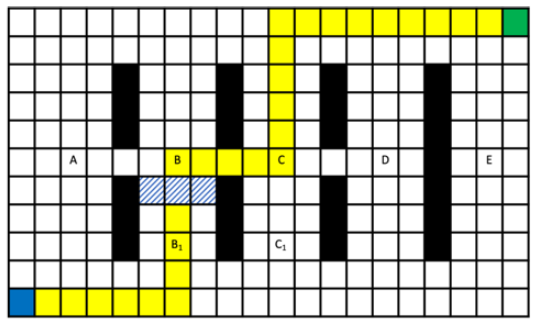
\includegraphics[width=\linewidth]{blockedAisleB.png}
					\caption{An obstacle in aisle B obstructs the planned path of the robot.}
					\label{fig:blockedAisleB}
				\end{subfigure}
				\caption{Illustration of case where robot observes an obstruction to it's planned path.}
				\label{fig:task1_1Figures}
			\end{figure}

			The scenario that we will be analysing is the case shown in Fig. \ref{fig:originalPlannedPath}. The robot is required to go from a cell $I$ to a cell $G$. These cells are marked blue and green in Fig. \ref{fig:originalPlannedPath} respectively. The figure also shows the original planned path that the robot computed going down aisle B. However, once the robot turns into aisle B it observes that the aisle is blocked. This observation is done at the point when the robot reaches the cell labelled $B_{1}$. At this point the robot can either decide to wait until the obstruction clears or it can re-plan a path. Once the robot observes the obstacle, the time the robot must wait for the obstacle to clear may be represented by the expression in Eq. \ref{eqn:waitTime}. 

			\begin{equation}
				T=\frac{0.5}{\lambda_{B}}+\widetilde{T}
				\label{eqn:waitTime}
			\end{equation}

			The wait time is dependent on $\lambda_{B}$ and a random variable $\widetilde{T}$. The random variable $\widetilde{T}$ is sampled from a exponential distribution with a rate parameter of $2\lambda_{B}$. The probability density function (PDF) for $\widetilde{T}$ is shown in Eq. \ref{eqn:waitTimePDF}. 

			\begin{equation}
				f(t) = 
				\begin{cases}
				\lambda e^{-\lambda t} & \quad t \geq 0 \\
				0 & \quad t < 0
				\end{cases}
				\label{eqn:waitTimePDF}
			\end{equation}
			where, rate parameter $\lambda = \dfrac{\lambda_{B}}{0.5}$. 
			
			As previously mentioned, the robot has two options to choose from: to wait for the obstacle to clear, or to re-plan and execute the new path. The two are different policies the robot must choose from. We use the symbol $\pi$ to denote a policy. A policy is a mapping from the world state to an action the robot can execute.
			\\
			\\
			Let us assume that if the robot decides to wait the total path length (number of cells) will be $K_1$ while if the robot decides to re-plan and execute the total path length will be $K_2$. We let the quantity $K$ equal to the larger value between $K_1$ and $K_2$. Now we may write the policy for the robot to wait as $\pi_{K}^{1}$ and the policy for re-planning as $\pi_{K}^{2}$. These policies are padded correspondingly to produce actions $\textbf{u}_{K}^{1}$ and $\textbf{u}_{K}^{1}$ that are padded with zero-cost state preserving actions.
			\\
			\\
			To see which policy is better on average, we consider the expected value of the cost function for both cases. The case when policy $\pi_{K}^{1}$ is chosen is characterized by the inequality shown in Eq. \ref{eqn:costExpectation}.

			\begin{equation}
				\mathbb{E}\left[L\left(\pi_{K}^{1}\right)\right] \leq \mathbb{E}\left[L\left(\pi_{K}^{2}\right)\right]
				\label{eqn:costExpectation}
			\end{equation}

			\begin{figure}[H]
				\centering
				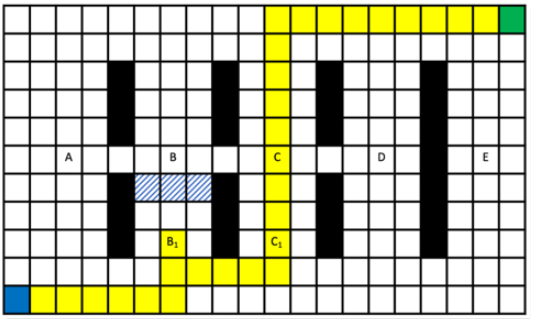
\includegraphics[scale=0.6]{images/replannedPathAisleB.png}
				\caption{The path for the re-plan policy $\pi_{K}^{2}$ which bypasses aisle B and goes down aisle C.}
				\label{fig:replannedPathAisleB}
			\end{figure}

			We can see from Fig. \ref{fig:originalPlannedPath} that the cost of the original planned path is given by the expression in Eq. \ref{eqn:waitingPolicyCost}. In this equation, the terms $L_{XY}$ denote the cost of the shortest path between cell $X$ and cell $Y$. Additionally, the term $L_{W}$ represents the cost of waiting 1 unit of time.
			
			\begin{equation}
				L\left(\pi_{K}^{1}\right) = L_{IB_{1}} + TL_W + L_{B_{1}B} + L_{BC} + L_{CG}
				\label{eqn:waitingPolicyCost}
			\end{equation}

			From Fig. \ref{fig:replannedPathAisleB} which shows the re-planned path, we can also see that the cost of this path is equal to the expression in Eq. \ref{eqn:replanPolicyCost}

			\begin{equation}
				L\left(\pi_{K}^{2}\right) = L_{IB_{1}} + L_{B_{1}C_{1}} + L_{C_{1}C} + L_{CG}
				\label{eqn:replanPolicyCost}
			\end{equation}

			Substituting the expressions in Eq. \ref{eqn:waitingPolicyCost} and Eq. \ref{eqn:replanPolicyCost} into Eq. \ref{eqn:costExpectation}. We obtain the inequality shown in Eq. \ref{eqn:costExpectation1}

			\begin{equation}
				\begin{split}
					\mathbb{E}\left[L_{IB_{1}} + TL_W + L_{B_{1}B} + L_{BC} + L_{CG}\right] & \leq \mathbb{E}\left[L_{IB_{1}} + L_{B_{1}C_{1}} + L_{C_{1}C} + L_{CG}\right] \\
					L_{IB_{1}} + \mathbb{E}\left[T\right] L_W + L_{B_{1}B} + L_{BC} + L_{CG} & \leq L_{IB_{1}} + L_{B_{1}C_{1}} + L_{C_{1}C} + L_{CG} \\
					\mathbb{E}\left[T\right] & \leq \frac{L_{B_{1}C_{1}} + L_{C_{1}C} - L_{B_{1}B} - L_{BC}}{L_W}
				\end{split}
				\label{eqn:costExpectation1}
			\end{equation}

			The quantity $\mathbb{E}\left[T\right]$ is the expected value for the time the robot has to wait for the obstacle to clear. As we know the distribution that the variable is sampled from we can compute the expected value. The expected value for the time taken is given by the expression found in Eq. \ref{eqn:waitTimeExpectation}

			\begin{equation}
				\begin{split}
					\mathbb{E}\left[T\right] & = \mathbb{E}\left[\frac{0.5}{\lambda_{B}}+\widetilde{T}\right] \\
					& = \frac{0.5}{\lambda_{B}} + \mathbb{E}\left[\widetilde{T}\right] \\
					& = \frac{0.5}{\lambda_{B}} + \int_{0}^{\infty}t\frac{\lambda_{B}}{0.5}e^{-\frac{\lambda_{B}}{0.5}t} dt \\
					& = \frac{0.5}{\lambda_{B}} + \frac{\lambda_{B}}{0.5}\left[-\left(t\right) \left(\frac{0.5}{\lambda_{B}}e^{-\frac{\lambda_{B}}{0.5}t}\right) - \int_{0}^{\infty}\frac{0.5}{\lambda_{B}}e^{-\frac{\lambda_{B}}{0.5}t} dt \right]_{0}^{\infty}\\
					& = \frac{0.5}{\lambda_{B}} + \frac{\lambda_{B}}{0.5} \times \frac{0.5}{\lambda_{B}} \left[-te^{-\frac{\lambda_{B}}{0.5}t} + \left[-\frac{\lambda_{B}}{0.5}e^{-\frac{\lambda_{B}}{0.5}t}\right]\right]_{0}^{\infty} \\
					& = \frac{0.5}{\lambda_{B}} + \left[-te^{-\frac{\lambda_{B}}{0.5}t} - \frac{\lambda_{B}}{0.5}e^{-\frac{\lambda_{B}}{0.5}t}\right]_{0}^{\infty} \\
					& = \frac{0.5}{\lambda_{B}} + \left[\lim_{t \to \infty} -te^{-\frac{\lambda_{B}}{0.5}t} + \frac{0.5}{\lambda_{B}}e^{-\infty} + 0 + \frac{\lambda_{B}}{0.5}e^0\right] \\
					& = \frac{0.5}{\lambda_{B}} +\frac{0.5}{\lambda_{B}} = \frac{1}{\lambda_{B}}
				\end{split}
				\label{eqn:waitTimeExpectation}
			\end{equation}

			Substituting the expression from Eq. \ref{eqn:waitTimeExpectation} into Eq. \ref{eqn:costExpectation1} we obtain the expression in Eq. \ref{eqn:lambdaInequality}. The right-hand side of the inequality in Eq. \ref{eqn:lambdaInequality} represents the smallest possible value for $\lambda_{B}$ for which the waiting policy $\pi_K^1$ is a better option than the re-plan policy $\pi_K^2$. The inequality also takes into consideration the constraint that $\lambda_{B} > 0$ and negates the solution when $\lambda_{B} < 0$.

			\begin{equation}
				\begin{split}
					\frac{1}{\lambda_{B}} & \leq \frac{L_{B_{1}C_{1}} + L_{C_{1}C} - L_{B_{1}B} - L_{BC}}{L_W} \\	
					\lambda_{B} & \geq \frac{L_W}{L_{B_{1}C_{1}} + L_{C_{1}C} - L_{B_{1}B} - L_{BC}}
				\end{split}
				\label{eqn:lambdaInequality}
			\end{equation}

		\subsection{Policy Selection at Start}
		\label{sec:policySelectionAtStart}
		
			\begin{figure}[H]
				\centering
				\begin{subfigure}{.4\textwidth}
					\centering
					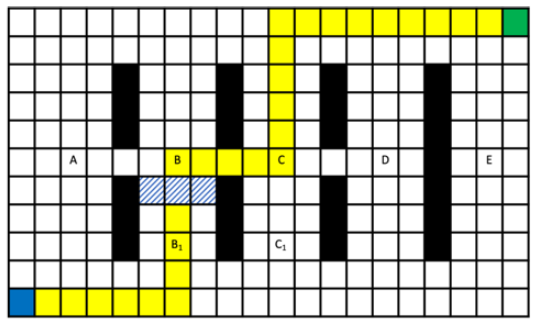
\includegraphics[width=\linewidth]{blockedAisleB.png}
					\caption{The scenario where the robot decides to go down Aisle B, encounters an obstacles and waits for it to clear.}
					\label{fig:plannedPathAisleB}
				\end{subfigure}
				\begin{subfigure}{.4\textwidth}
					\centering
					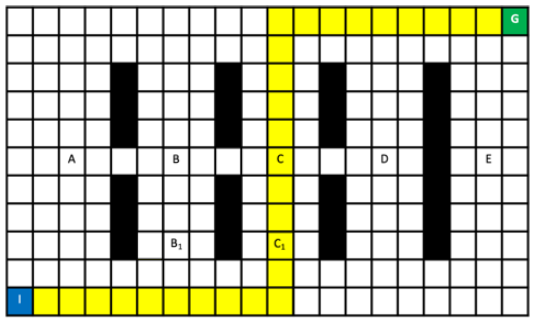
\includegraphics[width=\linewidth]{plannedPathAisleC.png}
					\caption{The scenario where the robot decides to avoid Aisle B completely due to the obstacle.}
					\label{fig:plannedPathAisleC}
				\end{subfigure}
				\caption{The different policies the robot can pick from at the beginning.}
				\label{fig:task1_2Figures}
			\end{figure}
			
			 Instead of reacting to the obstacle as the robot observes it, the robot may also make a decision before it start to move. The robot has knowledge of where the obstacles will be and the probability distribution for the wait time. Depending on the probabilities involved, the robot may decide to avoid the obstacle altogether instead of going the route with the obstacle and wait. In the case of the warehouse example with 5 aisles, and one obstacle in aisle B, the two policies are to choose to travel down aisle B and wait if an obstacle is present (illustrated in Fig. \ref{fig:plannedPathAisleB}) or to avoid aisle B and plan directly along aisle C (illustrated in Fig. \ref{fig:plannedPathAisleC}). Similar to the approach in \S \ref{sec:policySelectionWhenObstacleIsObserved}, we may denote the policy that goes down aisle B as $\pi_{K}^{1}$ and the policy that goes down aisle C as $\pi_{K}^{2}$. Once again these are padded with zero-cost state preserving actions so as to be of the same dimension. 
			\\
			\\
			We can see from Fig. \ref{fig:plannedPathAisleB} that the cost of policy that goes down aisle B, $\pi_{K}^{1}$, can cause 2 different scenarios: 
			\begin{itemize}
				\item Drive down aisle B and wait for the obstacle to move. The cost of this scenario is given by the expression:
				\begin{equation}
				L(\pi_k^1) = L_{IB_1}+TL_W+L_{B_1B}+L_{BC}+L_{CG}
				\label{eqn:waitPolicyCostStart1}
				\end{equation}
				\item Drive down aisle B, encounter an obstacle and reroute via aisle C.The cost of this scenario is given by the expression:
				\begin{equation}
				L(\pi_k^1) = L_{IB_1}+TL_W+L_{B_1B}+L_{BC}+L_{CG}
				\label{eqn:waitPolicyCostStart2}
				\end{equation}
			\end{itemize}
			
			The cost of the policy $\pi_{K}^{2}$, which associates to the robot deciding to drive down directly via aisle C is given by the expression in Eq. \ref{eqn:aisleCPolicyCostStart}.
			
			\begin{equation}
			L(\pi_k^2) = L_{IC}+L_{CG}
			\label{eqn:aisleCPolicyCostStart}
			\end{equation}
			
			As we are concerned with the average case scenario we compare the expected value of the loss function just as we did in section \ref{sec:policySelectionWhenObstacleIsObserved}. $\pi_{K}^{2}$ will be chosen over $\pi_{K}^{1}$ if the expected value of it's cost is lower as shown by Eq. \ref{eqn:expectationInequality}.
			
			\begin{equation}
			\mathbb{E}\left[L\left(\pi_{K}^{2}\right)\right] \leq \mathbb{E}\left[L\left(\pi_{K}^{1}\right)\right]
			\label{eqn:expectationInequality}
			\end{equation}
			
			Given that we can intuitively think of the cost associated to the second scenario of driving down aisle B given by eq. (\ref{waitPolicyCostStart2}) is a much longer path than directly driving down aisle C we can eliminate that from the comparison. Then, substituting the loss functions from eq. (\ref{eqn:waitPolicyCostStart}) and (\ref{eqn:aisleCPolicyCostStart}) into the inequality in eq. (\ref{eqn:expectationInequality}), we obtain the result shown in eq. (\ref{eqn:expectationInequality1}).
			
			\begin{equation}
			\begin{split}
			\mathbb{E}[L_{IC}+L_{CG}] \leq \mathbb{E}[L_{IB_1}+TL_W + L_{B_1B}+L_{BC}+L_{CG}] \\
			\mathbb{E}[T]L_W \geq L_{IC}-L_{IB_1}-L_{B_1B}-L_{BC}\\
			\mathbb{E}[T] \geq \frac{L_{IC}-L_{IB_1}-L_{B_1B}-L_{BC}}{L_W}
			\end{split}
			\label{eqn:expectationInequality1}
			\end{equation}
			
			
			
			By substituting the expected value for $T$ found in eq. (\ref{eqn:waitTimeExpectation}) we obtain a constraint for $\lambda_B$ as shown in eq. (\ref{eqn:constraintPlanAtStart}). The right hand side of the final inequality in eq. (\ref{eqn:constraintPlanAtStart}) represents the largest value for $\lambda_B$ for which the robot will decide to go directly down aisle C avoiding aisle B. 
			
			\begin{equation}
			\begin{split}
			\frac{1}{\lambda_B} \geq \frac{L_{IC}-L_{IB_1}-L_{B_1B}-L_{BC}}{L_W}\\
			\lambda_B \leq \frac{L_W}{L_{IC}-L_{IB_1}-L_{B_1B}-L_{BC}}
			\end{split}
			\label{eqn:constraintPlanAtStart}
			\end{equation}

		\subsection{Considering the Probability of the Obstacle Being Present}
		In reality, the obstacle would not be present there all the time. This can be taken into account using a probability, say $p_B$ associated with the scenario that the obstacle is present\footnote{This means that the probability that the obstacle is absent can be given by $ (1-p_B) $}. This means that the cost of waiting ($ L(\boldsymbol{x}_k,\boldsymbol{u}_w) $) at the obstacle to move for T stages will now become,
		\begin{equation}
			L(\boldsymbol{x}_k,\boldsymbol{u}_w) = p_B T L_w
		\end{equation}
		where, T is represented by eq.(\ref{eqn:waitTime}). 
		
		Therefore, the expected wait time $T'$ can be calculated as,
		\begin{equation}
		\begin{aligned}
		T'&= \frac{L(\boldsymbol{x}_k,\boldsymbol{u}_w)}{L_w}
		&= p_B \mathbb{E}[T]
		&= \frac{p_B}{\lambda_B}
		\end{aligned}
		\label{eq:expected-time-prob}
		\end{equation}
		where, $\mathbb{E}[T]$ is given by eq. \ref{eqn:costExpectation1}
		
		Given eq. (\ref{eq:expected-time-prob}), 
		\begin{equation}
		\begin{split}
		\frac{p_B}{\lambda_B} \geq \frac{L_{IC}-L_{IB_1}-L_{B_1B}-L_{BC}}{L_W} \\
		p_B \geq \frac{\lambda_B\left(L_{IC}-L_{IB_1}-L_{B_1B}-L_{BC}\right)}{L_W}
		\end{split}
		\label{eqn:constraintPlanAtStartwithProbability}
		\end{equation}
		
		
		
		\subsection{Considering Multiple Obstacles}

	%%%%%%%%%%%%%%%%%%%%%%%%%%%%%%%%%%%%%%
	
	%%%%%%%%%%% PART 2 %%%%%%%%%%%%%%%%%
	\section{ROS Implementation}

		

	%%%%%%%%%%%%%%%%%%%%%%%%%%%%%%%%%%%%%%
	
	\bibliographystyle{IEEEtran}
	\bibliography{references}

	%%%%%%%%%%%%%%%%%%%%%%%%%%%%%%%%%%%%%%

	\newpage
	\appendix
	\appendixpage
	\addappheadtotoc
	
\end{document}